\chapter[Ferramentas de Gerência de Requisitos]{Ferramentas de Gerência de Requisitos}

Ferramentas de gerência de requisitos foram feitas com o intuito de auxiliar os responsáveis pelo desenvolvimento do software a gerir os requisitos. Em geral, essas ferramentas armazenam, coletam, aplicam mudanças, inserem, atualizam e excluem, mantém versões dos requisitos. Apesar disso, as ferramentas possuem divergências entre suas funcionalidades, assim, cada programa atende a realidade de uma empresa \cite{ananias2009}.

\section{Análise das ferramentas}

\subsection{RallyDev}
O RallyDev é uma ferramenta comercial que da suporte a gestão de projetos de desenvolvimento de software. A ferramenta dá suporte a abordagens ágeis podendo se fazer gestão ao nível dos requisitos, dos testes, dos problemas e do planeamento e monitorização \cite{rallyDev}. Algumas das funcionalidades.

A ferramenta oferece:
\begin{itemize}
    \item Gerar relatórios e obter relatórios de progresso como burndown, velocity.
    \item Gestão de riscos visualizar blocos, defeitos, marcos e dependências.
    \item Gerenciamento de teste, integrar o planejamento funcional e testes de regressão.
    \item Release planning, criar roteiros realistas que permitam equilibrar o escopo, dependências e riscos.
    \item Rastreamento de lançamento, orientar entrega de recursos e lançamentos para atender às metas de negócios.
    \item Utilização de plugins 
    \item Integração com outras ferramentas de requisitos corporativos e Qualidade e software CRM. \newline Exemplos de ferramentas que o RallyDev faz integração: Bugzilla e Visual Studio.
\end{itemize}
               
Essas outras funcionalidades reforçam as tarefas de uma ferramenta de gerenciamento de requisitos já mencionadas, além de proporcionar algumas outras facilidades ao usuário.
\begin{figure}[H]
    \centering
    \label{rallydev}
    \caption[Tela do software RallyDev]{Tela do software RallyDev. fonte: \url{https://www.rallydev.com/sites/default/files/Feature\%20Summary\%20for\%20Requirements\%20Management_0.gif}}
    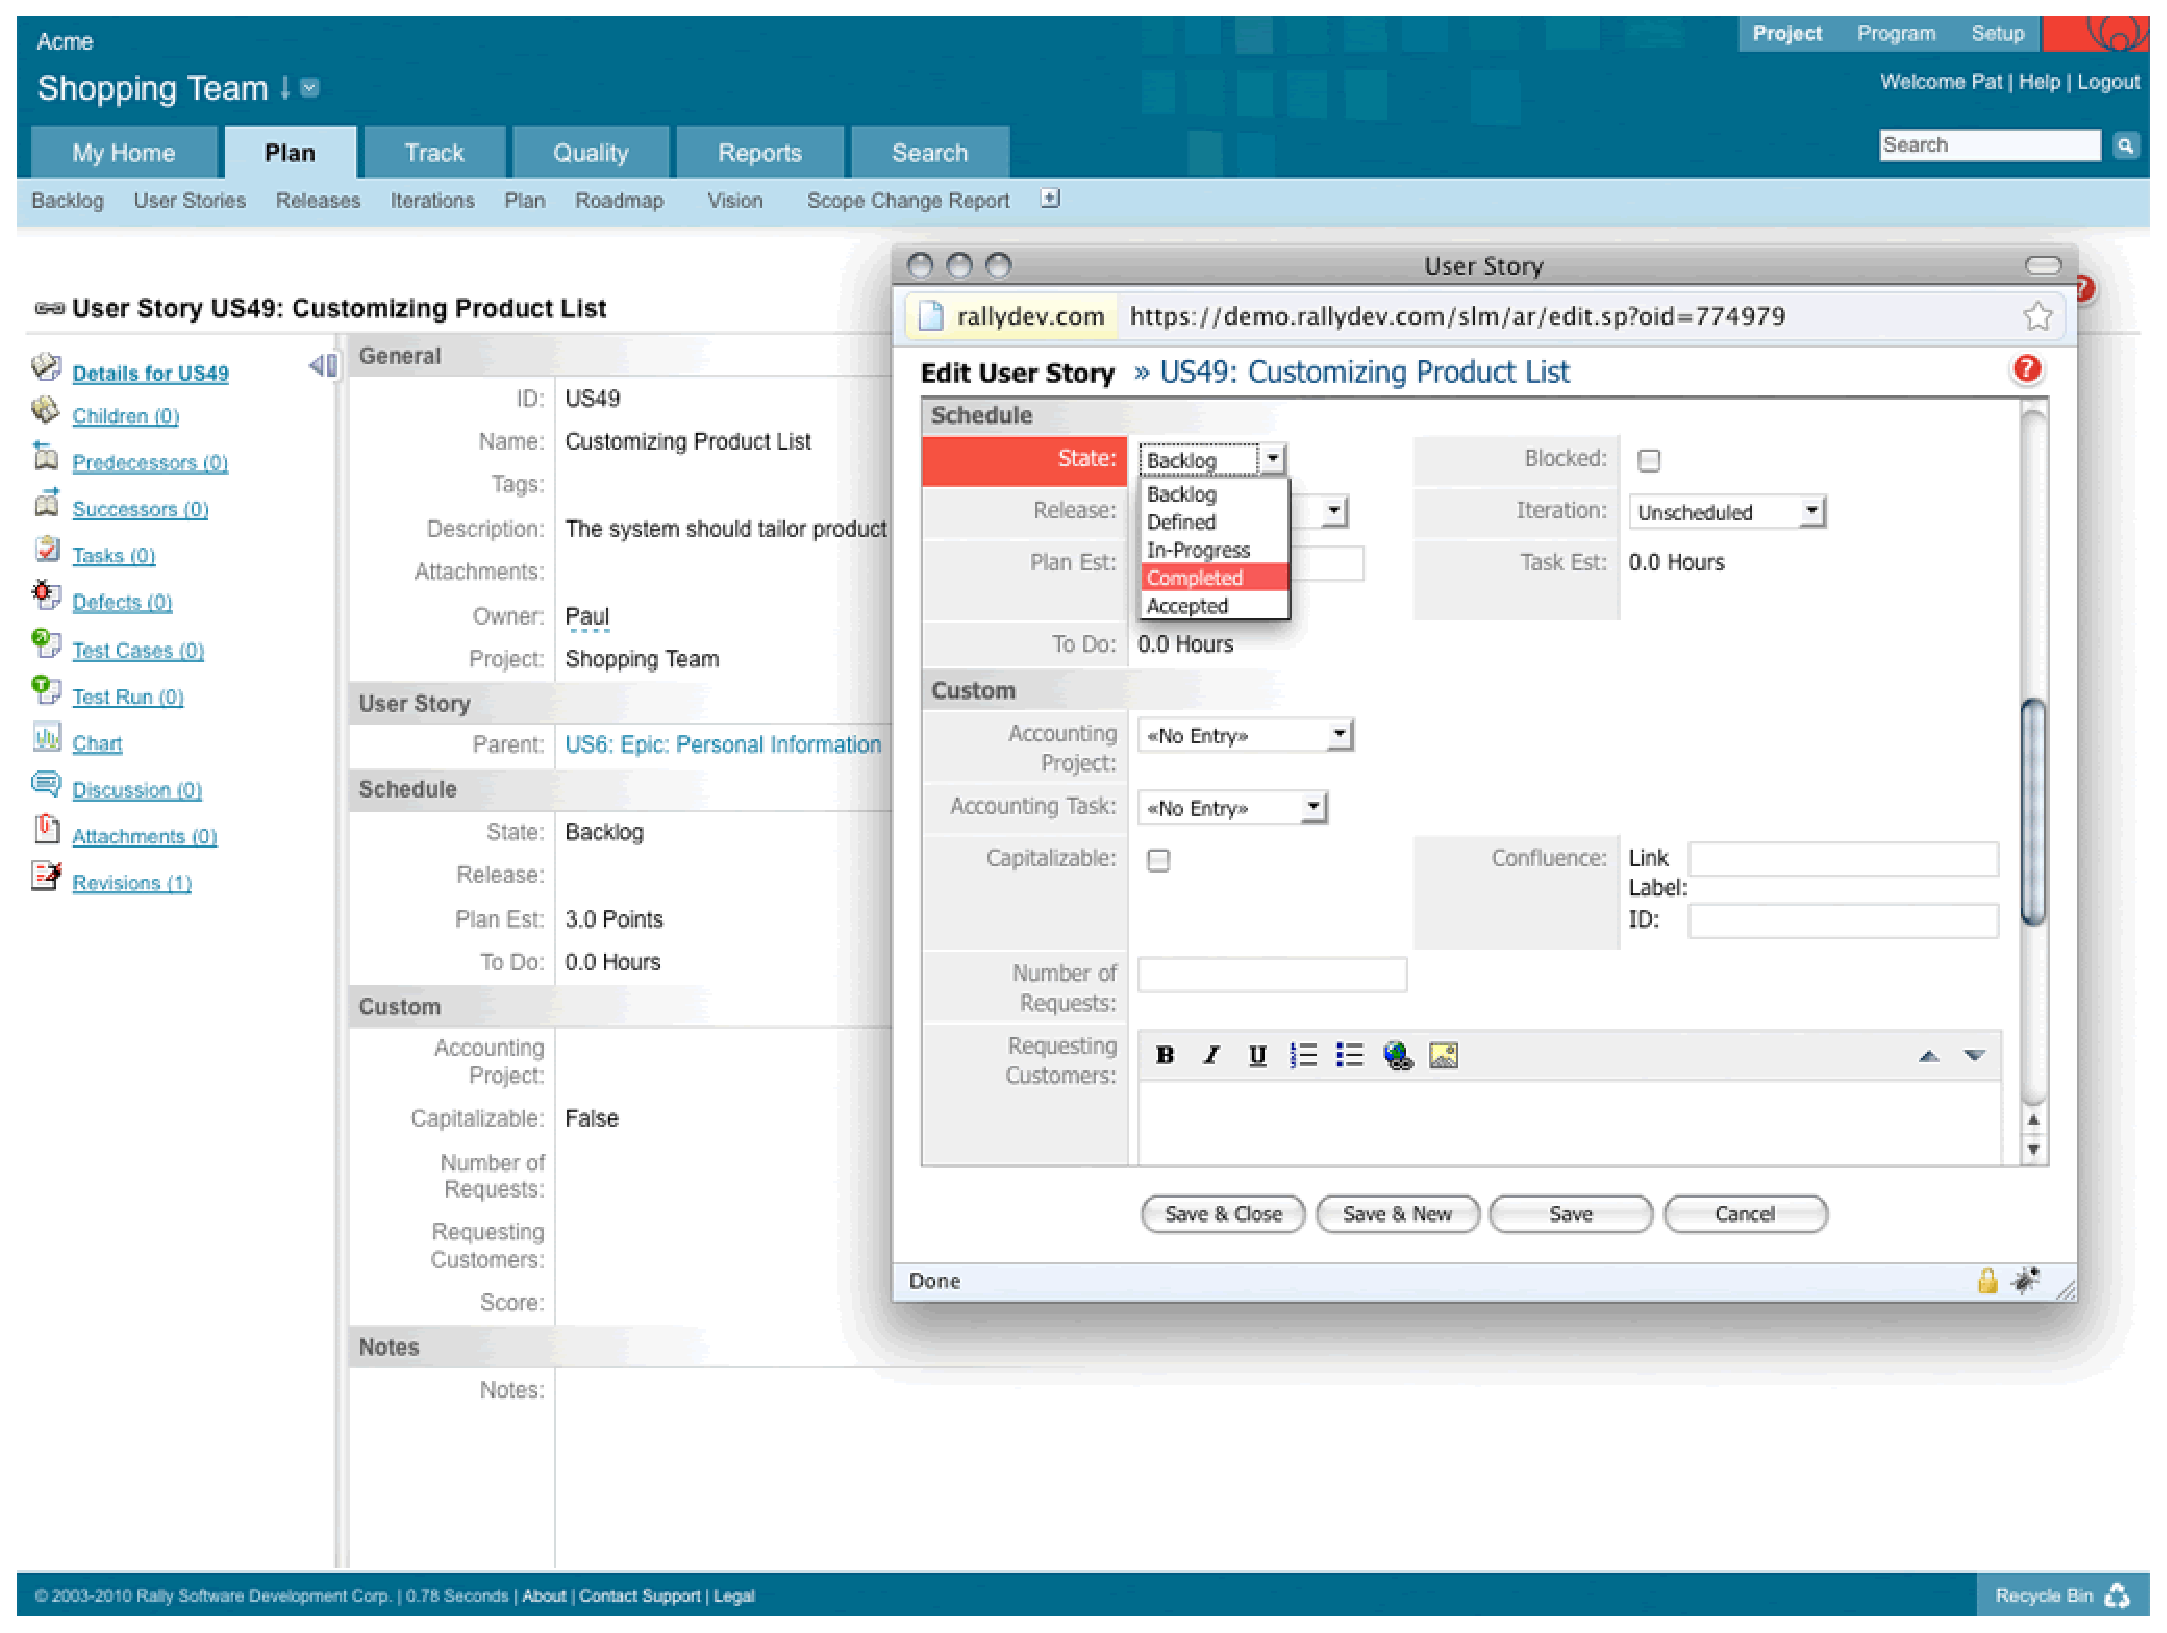
\includegraphics[keepaspectratio=true,scale=0.4]{figuras/rallydev.eps}
\end{figure}

\subsection{Jira}

Jira é um software comercial pago desenvolvido pela empresa Australiana Atlassian. É uma ferramenta que permite o monitoramento de tarefas e acompanhamento de projetos, bem como para acompanhamento e reporte de defeitos em projetos de qualquer natureza. Esta ferramenta é baseada em Java EE que operam em vários Bancos de dados sendo estes: PostgreSQL, MySQL, Oracle e SQL Server para as versões 2005, 2008, 2012. O Jira é multiplataforma operando nos seguintes sistemas operacionais: Linux, Windows e Solaris \cite{jira2016}. 

O Jira possui alguns plugins para acompanhamento do progresso do projeto, com gráficos de pizza, gráficos de barra, filtro por versão, filtro por status dentre outros. Exemplos de alguns plugins para o Jira: BigTemplate, Workflow Tools and Functions (WTF) e em especial o plugin GreenHopper, que possibilita o usuário gerenciar projetos ágeis. 

A ferramenta oferece:
\begin{itemize}
    \item Possibilidade de registrar uma tarefa, classificar como bug, features ou itens de backlog;
    \item Incluir numa determinada versão;
    \item Indicar que a tarefa está sendo executada, que já foi executada ou que nem começou e quem é responsável por ela. 
    \item Controle de acesso e segurança customizado.
    \item Gestão de defeitos e incidentes: funcionalidades para criação, detalhamento e descrição de defeitos  ou incidentes e acompanhamento de resolução.
    \item Gestão de projetos: criação e delegação de projetos e tarefas, com fluxos de processos personalizados para o acompanhamento dos projetos.
    \item Integração com ambientes de desenvolvimento. \textbf{Exemplos:} Eclipse, Visual Studio, IntelliJ, Netbeans, entre outros.
    \item Importação de dados de outras ferramentas populares. \textbf{Exemplo:} Mantis.
\end{itemize} 

O Jira atende as principais tarefas de uma ferramenta de gerenciamento de requisitos de software. Esta ferramenta pode ser utilizado via web tendo suporte para os seguintes browsers: Microsoft Internet, Explorer, Mozilla Firefox, Google Chrome e Safari. Também pode ser instalado em um desktop ou notebook. A ferramenta requer um banco de dados e o Oracle JDK para funcionar \cite{jira2016}.
\begin{figure}[H]
    \centering
    \caption[Tela do software Jira]{Tela do software Jira. fonte: \url{https://wac-cdn.atlassian.com/software/jira/main/01/columns/00/content/0/localUpload/Backlog@2x.png.png?cdnVersion=k}}
    \label{jiraFerramenta}
    \includegraphics[keepaspectratio=true,scale=0.2]{figuras/jira.eps}
\end{figure}

\subsection{Version One}

Ferramenta desenvolvida para auxiliar na gestão de projetos com processos ágeis, possuindo uma versão comercial e uma versão gratuita por um ano com limitações de número de usuários e recursos.

A ferramenta oferece \cite{versionOne}:
\begin{itemize}
    \item Incorporação dos conceitos relevantes aos princípios ágeis: planeamento de releases e iterações, histórias de utilização, tarefas e burndown;
    \item Associação de itens do Backlog a objectivos estratégicos de negócio e a grupos de funcionalidades; 
    \item Suporte a geração automática de histórias ou \textit{defects} a partir de sugestões submetidas pelo cliente; 
    \item Suporte a matriz de rastreabilidade;
    \item Integração para APIs, Java, .NET SDK;
    \item Geração de relatórios;
    \item Suporte multiplataforma e suporte Web;
    \item Visualização em gráficos.
\end{itemize}

\begin{figure}[H]
    \centering
    \caption[Tela do software VersionOne]{Tela do software VersionOne. fonte: \url{https://www.versionone.com/wp-content/uploads/2015/07/limit-your-teams-work-in-process-wip-lg.jpg}}
    \label{versionOneFerramenta}
    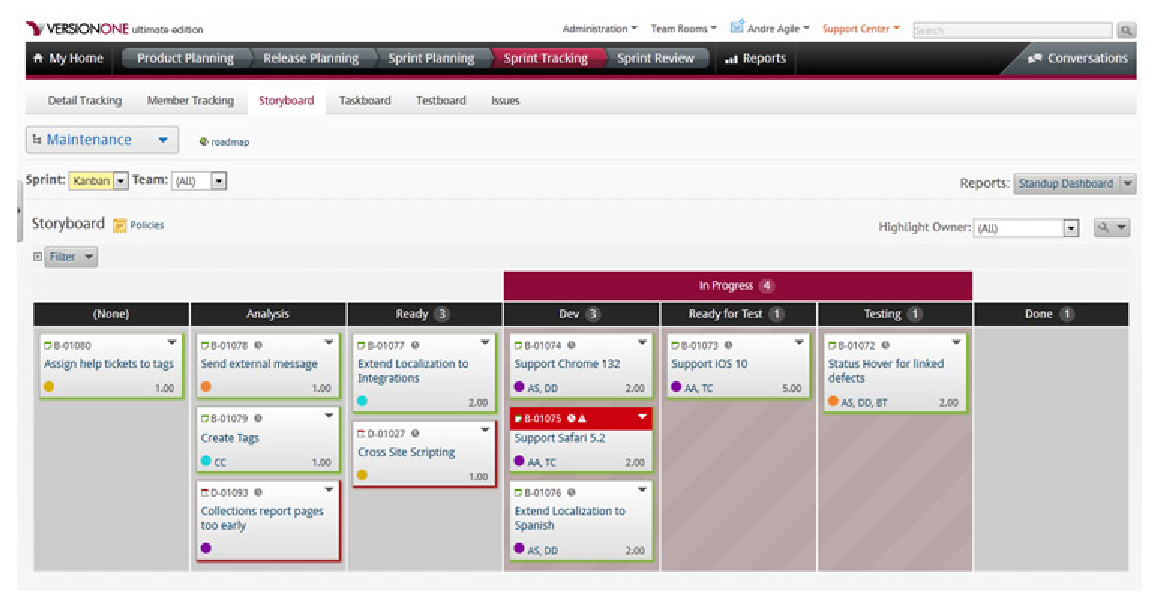
\includegraphics[keepaspectratio=true,scale=0.8]{figuras/versionOne.eps}
\end{figure}

\section{Escolha da ferramenta}
    
Para a escolha da ferramenta, foi elaborado critérios para avaliar as ferramentas selecionadas a base de pesquisas e indicações para garantir que a opção escolhida supre as necessidades do nosso contexto de negócio. A escolha dos critérios são baseadas nas atividades que desempenharemos no nosso processo, porém foi também levado em consideração os critérios \cite{hoffmann2004}.

\subsection{Ferramenta escolhida}

Existem duas classificações importantes para a escolha de uma ferramenta de gerenciamento de requisitos, requisitos de desenvolvedores e requisitos de projetos administradores \cite{hoffmann2004}. Os requisitos de projetos administradores são para projetos de larga escala, e como o projeto em questão é um projeto de pequena e média escala, logo só serão tratados os requisitos de desenvolvedores.

\subsubsection{Critérios e metodologia de análise}

Para a escolha da ferramenta, foram escolhidos critérios baseados no Hoffmann (2004) e critérios elaborados pela equipe para se adequarem as necessidades da disciplina de engenharia de requisitos.
Para cada critério especificado, foi adotado um grau de prioridade para classificar a importância do critério para a escolha da ferramenta. Assim, é definido: 
\begin{description}
    \item '+++' - para alta prioridade; 
    \item '++' - média prioridade; 
    \item '+' - baixa prioridade;
\end{description}

A contagem para determinar a escolha da ferramenta, será definido pela soma de unidades de '+', em que cada um desse representa uma unidade de pontuação, que a ferramenta acumulou após a análise de todos os critérios estabelecidos.

\begin{itemize}
    \item \textbf{A abordagem adotada(+++):} a ferramenta deve ter suporte para a abordagem ágil, ou seja, dando suporte a Histórias de Usuário; Priorização de atividades; Backlog dentre outras atividades que o processo demanda relacionado a abordagem ágil;     
    \item \textbf{Matriz de Rastreabilidade(+++):} a ferramenta deve dar suporte a rastreabilidade dos requisitos às suas origens e os rastreamento durante todo o ciclo de vida do projeto. A ferramenta deve permitir a rastreabilidade através de links entre os requisitos, devendo ser possível seguir através desses links diretamente em ambos as direções \cite{hoffmann2004}.     
    \item \textbf{Acesso Web(+):} a ferramenta deve dar suporte a uma interface web para que não seja necessário instalar um aplicativo no computador para cada usuário que fará uso dela \cite{hoffmann2004}. Devendo também ter uma interface intuitiva e fácil de se manusear. O Jira oferece interface web intuitiva e fácil de utilizar.
    \item \textbf{Gestão de mudanças(++):} a ferramenta deve dar suporte para a gerenciamento de mudanças com base nas atividades desenvolvidas para lidar com essas modificações. Assim, com suporte ao gerenciamento de mudanças possibilita a redução de erros de forma significativa \cite{hoffmann2004}.
    \item \textbf{Comentários(+):} Deve permitir adicionar comentários aos requisitos, estes são para adicionar esclarecimentos necessários aos requisitos que não são simples de entender ou que usem referências externas \cite{hoffmann2004}.
    \item \textbf{Geração de relatórios(+):} a ferramenta deve dar suporte para a documentação de atividades realizadas e  prover a possibilidade de outros formatos de arquivos para programas externos a ferramenta.
    \item \textbf{Nível de documentação(+++):} o processo escolhido exige que seja permitido documentar os requisitos em quatro níveis: temas estratégicos, épicos, features e histórias de usuário.
\end{itemize}

A tabela a seguir define se a ferramenta atinge os critérios definidos. É avaliado se a ferramenta alcança as espectativas da equipe em relação ao critério adotado, assim como o grau de satisfação em relação ao comparativo entre as outras ferramentas. Isso quer dizer que, a ferramenta analizada não receber um 'X' indicando alcance do critério, não indica que a ferramenta não tenha tal funcionalidade e sim que não atendeu os critérios totalmente como era esperado.

\begin{table}[H]
    \centering
    \label{comparaFerramentas}
    \caption{Comparação entre ferramentas}
    \begin{tabular}{l|c|c|c}
        \hline
        Critérios & Jira &  RallyDev & VersionOne \\ [6pt]
        \hline
        Abordadem adotada(+++) & X & X & X\\
        \hline
        Matriz de rastreabilidade(+++) & X & - & X \\
        \hline
        Acesso Web(+) & X & X & X \\
        \hline
        Gestão de mudanças(++) & X & - & X\\
        \hline
        Comentários(+) & X & - & X \\
        \hline
        Geração de relatórios(+) & X & X & X \\
        \hline
        Soma dos pontos & 14 & 5 & 14 \\
        \hline
    \end{tabular}
\end{table}

Após a visualização do resultado na tabela contendo os critérios utilizados como base para a escolha da ferramenta. Constatou-se um empate entre as ferramentas Jira e VersionOne. Utilizando como critério de desempate o quesito a interface gráfica do software a ferramenta que se destacou foi o Jira. Portanto, a ferramenta que será utilizada para a gerência de requisitos é o Jira.
